\documentclass[11pt]{article}
\usepackage[a4paper,margin=1in]{geometry}
\usepackage{amsmath,amssymb}
\usepackage{booktabs}
\usepackage{graphicx}
\usepackage{microtype}
\usepackage[colorlinks=true,linkcolor=blue,citecolor=blue,urlcolor=blue]{hyperref}
\usepackage{caption}
\captionsetup{font=small,labelfont=bf}

\title{\textbf{Diffusive and Bending Modes of the S\&P~500 Implied-Volatility Surface:\\ A Field-Theory Factor Model Tested Out of Sample}}
\author{Alexander~Pascal\\ Department of Physics, King's College London\\ \small\texttt{github.com/MichaelAafton/diffusion-modes-vol-surface}}
\date{September 2026}

\begin{document}
\maketitle

\begin{abstract}
\noindent We test whether the day-to-day dynamics of the S\&P~500 implied-volatility smile are consistent with a stochastic heat equation, using ten years (2015--2024) of OptionMetrics IvyDB volatility surfaces. A validated synthetic harness establishes the correct null prediction: for daily \emph{changes}, an Ornstein--Uhlenbeck mode obeys $\mathrm{Var}(\Delta f_k)=2V_k(1-e^{-\gamma_k\,dt})$, not the na\"ive $k^{-2}$ stationary law. Against this corrected null, pure diffusion is decisively rejected: across a matched-instrument parameter sweep, its spectral slope saturates at $p\le1.87$, versus $p\approx2.5$--$2.6$ observed in the tail of the real spectrum. A three-parameter composite model, an external volatility-level factor riding on a membrane with both tension and bending rigidity, $\gamma_k = Dk^2+\kappa k^4$, reproduces the full eight-point empirical spectrum. Formal calibration with block-bootstrap errors yields $D=0.69\;[0.29,1.25]$, $\kappa=0.011\;[0.006,0.020]$, and a diffusion-to-bending crossover $k^\ast=7.9\;[5.1,11.2]$ at the upper edge of the observable band ($\chi^2/\mathrm{dof}=3.6$). The sole significant residual is a mode-5 ``shelf'' ($z=-3.0$). In a chronological out-of-sample test (train through 2022-01-05, test through 2024-12-31), the three-parameter field theory predicts portfolio risk within $1\%$ of an empirical three-factor model on level, straddle, and risk-reversal exposures, while a butterfly portfolio loading precisely modes 3--5, exposes the same spectral residual in money terms, over-predicted $2.2\times$. The smile behaves as a stiff membrane plus an external level factor; where the picture fails is localised, twice measured, and characterised.
\end{abstract}

\section{Introduction}

The implied-volatility surface of a liquid index \cite{gatheral} is not static: it breathes daily, and the structure of that breathing determines the risk of every option portfolio. A long-standing physics-inspired proposal \cite{lecoz,bouchaud,cont}\footnote{The project was directly inspired by an unpublished presentation, \emph{A Data-Driven Factor Model for Option Risk}, by P.~Ioselevich (Capital Fund Management), for which no citable published version exists.} treats the surface as an elastic membrane: local supply--demand shocks perturb it, and an effective stiffness propagates and damps the perturbations. In its simplest form the proposal is a stochastic heat equation,
\begin{equation}
\partial_t p(z,t) \;=\; D\,\partial_z^2 p(z,t) + \xi(z,t),
\label{eq:spde}
\end{equation}
for the perturbation field $p$ on a moneyness axis $z$, with white noise $\xi$. Decomposed in Fourier modes, each amplitude is an independent Ornstein--Uhlenbeck (OU) process with relaxation rate $\gamma_k = Dk^2$, so the stationary mode variances scale as $k^{-2}$ and principal-component analysis (PCA) of surface co-movement should recover sinusoidal eigenvectors with a $k^{-2}$ eigenvalue decay.

This paper tests that prediction against real S\&P~500 (SPX) surfaces and reports, as its central results, the two places the prediction fails and the minimal extension that repairs them. The design principle throughout is that synthetic data is a \emph{validation harness}, never evidence: simulations prove the pipeline recovers known ground truth; only real data can support or falsify the physical hypothesis; and deviations from the diffusive picture are the scientific product, not a defect.

The contributions are:
\begin{enumerate}
\item \textbf{A corrected null hypothesis.} The $k^{-2}$ law governs mode \emph{levels}; PCA is necessarily run on daily \emph{changes} (for stationarity), whose spectrum obeys the OU increment law $\mathrm{Var}(\Delta f_k)=2V_k(1-e^{-\gamma_k dt})$: flat for slow modes, $\propto k^{-2}$ for fast ones. Testing real data against the wrong null materially changes conclusions (Sec.~\ref{sec:harness}).
\item \textbf{Falsification of pure diffusion.} Through a matched instrument (identical grid, horizon, differencing, and estimator for synthetic and real data), no diffusion constant reproduces the observed spectrum: full-spectrum slope saturates at $p\le1.78$ and tail slope at $p\le1.87$, versus real values of $2.99$--$3.20$ and $2.53$--$2.64$ (Sec.~\ref{sec:adjudication}).
\item \textbf{A three-parameter composite that works.} An external level factor plus a membrane with bending rigidity, $\gamma_k=Dk^2+\kappa k^4$, reproduces the eight-point spectrum, including an untuned match of the smallest eigenvalue. Formal calibration with block-bootstrap uncertainties places the diffusion-to-bending crossover at the top of the observable band (Sec.~\ref{sec:calibration}).
\item \textbf{An out-of-sample risk test through a regime change.} Trained before 2022 and tested on 2022--2024, the three-parameter theory matches a 36-parameter empirical factor model to within $1\%$ on three of four standard portfolios; the fourth (butterfly) independently rediscovers the calibration's one significant residual in money terms (Sec.~\ref{sec:oos}).
\end{enumerate}

Section~\ref{sec:theory} develops the theory, Sec.~\ref{sec:data} the data and instrument, and Sec.~\ref{sec:discussion} discusses limitations, the decision log, and future work.

\section{Theoretical framework}
\label{sec:theory}

\subsection{Modes, levels, and the increment law}

On a finite $z$-domain of length $L$ with the operator $\mathcal{L}$, the field decomposes onto the cosine basis $\varphi_k(z)=\sqrt{2/L}\cos\!\big(k\pi(z-z_{\min})/L\big)$, $k=1,\dots$ Each amplitude obeys an OU equation $\dot f_k = -\gamma_k f_k + \xi_k$, whose stationary variance is
\begin{equation}
V_k=\frac{\sigma^2}{2\gamma_k}.
\end{equation}
For pure diffusion $\gamma_k = Dk^2$, giving the $k^{-2}$ level spectrum. We consider the extended operator
\begin{equation}
\gamma_k \;=\; D k^{2} + \kappa k^{4},
\label{eq:operator}
\end{equation}
in which $\kappa$ is a bending rigidity (the operator of a stiff plate rather than a tense membrane). The two regimes exchange dominance at the crossover wavenumber
\begin{equation}
k^\ast=\sqrt{D/\kappa}.
\end{equation}

Volatility levels are nearly integrated (close to a random walk), so PCA is performed on daily changes $\Delta\sigma$, which are approximately stationary. The correct null for a change-based spectrum follows from the exact OU transition $f(t+dt)=f\,e^{-\gamma dt}+\eta$, $\eta\sim\mathcal N\!\big(0,V(1-e^{-2\gamma dt})\big)$: writing $a=e^{-\gamma dt}$ and using independence of $\eta$ from $f$,
\begin{equation}
\mathrm{Var}(\Delta f)\;=\;V(1-a)^2+V(1-a^2)\;=\;2V\big(1-e^{-\gamma\,dt}\big).
\label{eq:increment}
\end{equation}
Equation~\eqref{eq:increment} has two personalities: for slow modes ($\gamma dt\ll1$) it reduces to $\sigma^2 dt$, \emph{independent of} $k$, all slow modes take the same daily kick, flattening the spectrum's head, while fast modes ($\gamma dt\gg1$) decorrelate fully between observations and inherit the level law $2V_k\propto\gamma_k^{-1}$. Any inference that compares a change-based empirical spectrum with the level law conflates these regimes; correcting this changed our own conclusions materially (Sec.~\ref{sec:adjudication}).

\subsection{Composite model}

Empirically (Sec.~\ref{sec:spectrum}) one mode dominates changes with a near-uniform profile across $z$: the entire smile repricing with the volatility level. We model it as an \emph{external} scalar factor $f_0(t)$, an AR(1) with its own persistence and daily-kick variance $m$, added uniformly across $z$, rather than as the operator's $k{=}0$ mode. The model covariance of daily changes at grid points $z_i,z_j$ is then an exact finite sum,
\begin{equation}
\mathrm{Cov}(\Delta p_i,\Delta p_j) \;=\; \sum_{k=1}^{n} \varphi_k(z_i)\,\varphi_k(z_j)\; 2V_k\big(1-e^{-\gamma_k dt}\big)\;+\;m,
\label{eq:forward}
\end{equation}
which, correlation-normalised and eigendecomposed, yields deterministic model variance shares in microseconds, the forward model used for calibration, with no simulation in the optimisation loop.

\section{Data and instrument}
\label{sec:data}

\subsection{Source and design decisions}

Data are OptionMetrics IvyDB smoothed volatility surfaces (WRDS, \texttt{vsurfd}) for SPX (secid 108105), 2015--2024 ($\sim$2{,}500 trading days), pulled once and frozen to Parquet; spot from \texttt{secprd}. The surface supplies interpolated implied volatilities on fixed (maturity, delta) pillars together with the vendor's implied strike. We study the 30-calendar-day maturity slice. Key measurement decisions (the project maintains a numbered decision log, D1--D9; Appendix~\ref{app:dlog}):

\begin{itemize}
\item \textbf{Strike from vendor \texttt{impl\_strike}} (D1): self-consistent with the vendor's own surface construction; fewest moving assumptions.
\item \textbf{OTM-only stitching} (D2): retain $|\Delta|\le0.5$, so out-of-the-money puts populate $z<0$ and OTM calls $z>0$, each half of the axis represented by its liquid instrument.
\item \textbf{Calendar$\to$business-day conversion} (D3): surface maturities are calendar days; the pipeline's annualisation uses 252. Omitting the $252/365$ conversion silently shrinks every $z$ by $\sim$17\%.
\item \textbf{ATM-normalised moneyness} (D4): $z=\log(K/S)/(\sigma_{\mathrm{ATM}}\sqrt{T})$ with $\sigma_{\mathrm{ATM}}$ the per-(date, maturity) 50-delta call/put average. Normalising by each option's \emph{own} implied volatility makes the coordinate self-referential (a relabelling of delta); the ATM ruler is essential. The missing-$\sigma_{\mathrm{ATM}}$ path raises a hard error rather than falling back silently.
\end{itemize}

The delta-pillar grid ($|\Delta|\in[0.10,0.90]$, steps of $0.05$) maps to a usable window $z\in[-1.15,\,1.10]$; $13.3\%$ of raw rows (nearly all deep OTM puts) lie outside it. The pillar spacing supports $\approx8$ uniform bins, finer binning would manufacture resolution the instrument does not possess. \emph{The instrument's field of view and mode ceiling are properties of the data source, not of the market}; modes beyond $k\approx8$ are unobservable here.

\subsection{Panel construction}

Each option's $z$ is binned (\,8 uniform bins on $[-1.15,1.10]$\,) and implied vols averaged per (date, bin). A pre-registered 95\% coverage rule removes underpopulated bins; with clean numeric dtypes the panel is complete: $2{,}499\times8$ with no missing cells. (An earlier ``seven-bin'' panel was traced to vendor \texttt{Decimal}/\texttt{None} semantics silently corrupting coverage counts; column types are now coerced and unit-tested at the loader.) The analysis variable is the daily change $\Delta\sigma(z)$ (D5): stationary, matched to the harness-validated increment theory, and free of a hedging-frequency assumption. The caveat is inherited honestly: daily $\Delta\sigma$ at fixed $z$ differs from delta-hedged P\&L by gamma--theta carry, approximately a rank-one contamination concentrated in the level mode; interpretation of mode~1 carries an asterisk, modes $\ge2$ are robust.

\section{Validation harness}
\label{sec:harness}

The simulator evolves each mode by the \emph{exact} OU transition (zero discretisation error; unconditionally stable; initialised in stationarity), reconstructing $p(z,t)$ on the sampled cosine basis, with the level factor gated behind a configuration flag. The harness's purpose is falsification-grade validation of the pipeline: simulate, difference, run the \emph{identical} PCA, and require the empirical spectrum to match Eq.~\eqref{eq:increment}'s prediction, which it does to $\lesssim0.2$ percentage points per mode over $20{,}000$ synthetic days; the comparison is frozen as a permanent unit test. Two methodological rules emerged and are enforced throughout: (i)~\emph{aliasing control}: the number of simulated modes equals the number of grid points ($n_{\mathrm{modes}}=n_z$), since coarse sampling folds unrepresented high-$k$ variance into low modes and spuriously steepens spectra; (ii)~numerical guards are derived, not inherited, exponential underflow ($e^{-\gamma dt}\!\to\!0$) is the \emph{benign} exact-update limit (the mode redraws from its stationary law), unlike the instability of Euler--Maruyama at large $\gamma dt$.

\section{The empirical spectrum}
\label{sec:spectrum}

\begin{table}[t]
\centering
\caption{Empirical variance shares of daily $\Delta\sigma$ across 8 $z$-bins (2{,}498 changes), with moving-block bootstrap uncertainty (block $=25$ days, $1{,}000$ replicates).}
\label{tab:spectrum}
\begin{tabular}{cccc}
\toprule
Mode & Share & Boot.\ std & 95\% CI \\
\midrule
1 & 0.9150 & 0.0062 & [0.9043, 0.9286] \\
2 & 0.0493 & 0.0056 & [0.0358, 0.0552] \\
3 & 0.0164 & 0.0041 & [0.0109, 0.0260] \\
4 & 0.0067 & 0.0013 & [0.0058, 0.0108] \\
5 & 0.0064 & 0.0007 & [0.0046, 0.0071] \\
6 & 0.0029 & 0.0005 & [0.0020, 0.0041] \\
7 & 0.0019 & 0.0003 & [0.0014, 0.0024] \\
8 & 0.0014 & 0.0002 & [0.0010, 0.0018] \\
\bottomrule
\end{tabular}
\end{table}

Table~\ref{tab:spectrum} reports the correlation-matrix PCA of the real $\Delta\sigma$ panel. Structural findings:

\textbf{Mode shapes.} Mode~1 is uniform and positive across $z$ (entries $0.342$--$0.366\approx1/\sqrt8$; zero sign changes): the level mode, owning $91.5\%$ of daily-change variance. Mode~2 is a one-node see-saw, put wing against call wing: the skew mode. Both are stable under removal of the outermost put bin. Mode~3 fails the harmonic test: its shape is a dipole concentrated on the outermost bins that \emph{follows the boundary} when the edge bin is removed, and its node count is unstable ($2\to4$). Physics lives at a location; artifacts live at the boundary. Node-counting evidence for membrane structure therefore stops, by diagnosis rather than oversight, at mode~2. Both diagnostics are shown in Fig.~\ref{fig:modes}.

\begin{figure}[t]\centering
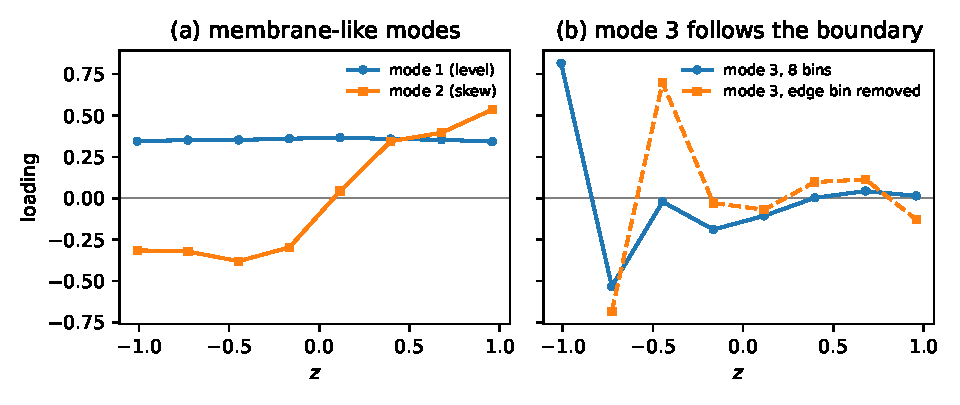
\includegraphics[width=.95\linewidth]{figures/fig2_modes.pdf}
\caption{(a) Modes 1--2 of the real $\Delta\sigma$ panel: uniform level and
one-node skew see-saw. (b) Mode 3 in the 8-bin panel and with the edge bin
removed: the dipole tracks the boundary, identifying it as an edge artifact.}
\label{fig:modes}
\end{figure}

\textbf{Slopes.} A log--log power-law fit $\lambda_k\sim k^{-p}$ over all modes gives $p=2.99$ (8 bins) and $3.20$ (edge bin excluded). Restricted to the tail (modes 2--8, fitted against their true wavenumbers), $p_{\mathrm{tail}}=2.53$ and $2.64$ respectively. The full-spectrum slope is substantially manufactured by mode~1's dominance; the tail slope is the operator-sensitive statistic. Both exceed the diffusive prediction, but by how much requires the matched-instrument null of the next section, since Eq.~\eqref{eq:increment} distorts any slope measured on daily changes. Fig.~\ref{fig:spectrum} shows the data, the calibrated fit of Sec.~\ref{sec:calibration}, and the falsified diffusive null in one frame.

\begin{figure}[t]\centering
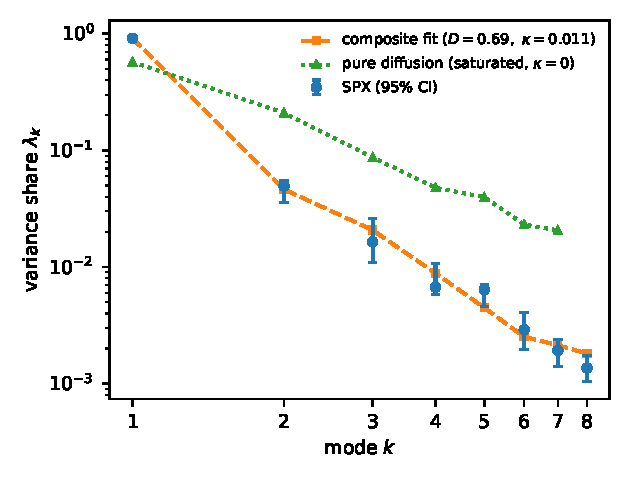
\includegraphics[width=.62\linewidth]{figures/fig1_spectrum.pdf}
\caption{Variance shares of daily $\Delta\sigma$: SPX with 95\% block-bootstrap
CIs, the calibrated composite model, and pure diffusion at its saturating best
(modes 1--7; its eighth eigenvalue is a structural zero of the 8-point
sampling). Mode 5 sits above the fit, the shelf residual of
Sec.~\ref{sec:calibration}.}
\label{fig:spectrum}
\end{figure}

\section{Operator adjudication}
\label{sec:adjudication}

\begin{table}[t]
\centering
\caption{Matched-instrument sweep: fitted slopes of synthetic spectra through the identical pipeline (8 bins on $[-1.15,1.10]$, 2{,}500 days, 5 seeds per cell, mean $\pm$ s.d.). Top: pure diffusion. Bottom: fixed $D=0.2$, increasing bending rigidity $\kappa$.}
\label{tab:sweep}
\begin{tabular}{cccccc}
\toprule
$D$ & $\kappa$ & $p_{\mathrm{full}}$ & $p_{\mathrm{tail}}$ & $k^\ast$ \\
\midrule
0.01 & 0 & $0.36\pm0.02$ & $0.42\pm0.03$ & $\infty$ \\
0.05 & 0 & $0.26\pm0.01$ & $0.34\pm0.02$ & $\infty$ \\
0.2  & 0 & $0.89\pm0.02$ & $1.12\pm0.04$ & $\infty$ \\
1    & 0 & $1.55\pm0.02$ & $1.73\pm0.04$ & $\infty$ \\
5    & 0 & $1.78\pm0.03$ & $1.87\pm0.04$ & $\infty$ \\
\midrule
0.2 & 0.01 & $1.54\pm0.02$ & $2.09\pm0.04$ & 4.47 \\
0.2 & 0.03 & $2.04\pm0.02$ & $2.74\pm0.04$ & 2.58 \\
0.2 & 0.1  & $2.64\pm0.02$ & $3.39\pm0.04$ & 1.41 \\
0.2 & 0.2  & $2.97\pm0.02$ & $3.69\pm0.04$ & 1.00 \\
0.2 & 0.3  & $3.15\pm0.02$ & $3.83\pm0.04$ & 0.82 \\
0.2 & 0.5  & $3.36\pm0.02$ & $4.00\pm0.03$ & 0.63 \\
0.2 & 1    & $3.62\pm0.02$ & $4.19\pm0.03$ & 0.45 \\
\bottomrule
\end{tabular}
\end{table}

Table~\ref{tab:sweep} answers the confound directly: what slope \emph{would} each candidate operator produce through this exact instrument?

\textbf{Diffusion is falsified twice.} Over the full $D$ sweep, the pure-diffusion slope saturates at $p_{\mathrm{full}}\le1.78$ and $p_{\mathrm{tail}}\le1.87$: the increment-law flattening can only pull slopes \emph{below} the level-law value of 2, never above. The real values ($2.99$--$3.20$; tail $2.53$--$2.64$) are unreachable, a gap of tens of standard errors, whether or not the suspect level mode is included.

\textbf{A single homogeneous $k^4$ operator is slope-sufficient but profile-falsified.} Bending rigidity does steepen spectra through the observable band, and $\kappa\approx0.2$--$0.3$ matches the real full-spectrum slope. But the match is an artifact of slope's shape-blindness: every homogeneous-operator spectrum in the sweep is \emph{concave} on log--log axes ($p_{\mathrm{tail}}>p_{\mathrm{full}}$), while the real spectrum is \emph{convex} ($p_{\mathrm{tail}}<p_{\mathrm{full}}$): a giant head over a gentle tail. At matched slope, the single-operator model mispredicts the mode-2 share sixfold (0.28 vs 0.049). Convexity of the real spectrum forces a two-component structure.

\textbf{The composite reproduces the eight-point profile.} With the level factor tuned to mode~1's share ($0.9157$ at daily kick s.d.\ $3.35$, hand stage) and the tail matched by $\kappa\approx0.02$ at $D=0.2$, the model tracks the real spectrum mode by mode, including two unforced agreements: the smallest eigenvalue, structurally zero for an 8-mode field on 8 points (rank deficiency), filled to $0.0013$ vs real $0.0014$ by the level factor as ninth variance source, and near-matching mid-tail shares. Residuals against synthetic seed noise alone appeared enormous (mode 3: $+31\sigma$) but shrink to honest size under the real spectrum's block-bootstrap errors (mode 3: $+1.9\sigma$, not significant), a caution recorded in the decision log: \emph{seed spread is not measurement error}.

\section{Calibration}
\label{sec:calibration}

Parameters are fitted by weighted least squares of the analytic forward model, Eq.~\eqref{eq:forward}, against the real shares: $\chi^2=\sum_{k=1}^{7}\big[(\hat\lambda_k-\lambda_k)/\sigma_k\big]^2$ with block-bootstrap $\sigma_k$; mode 8 is excluded as sum-determined (7 points, 3 parameters, $\mathrm{dof}=4$). Optimisation is Nelder--Mead in $(\log D,\log\kappa,\log m)$, positivity by construction, scale-symmetric uncertainty. Confidence intervals come from refitting each of the $1{,}000$ bootstrap spectra.

\begin{table}[t]
\centering
\caption{Calibrated composite model (bootstrap medians; 95\% CIs from bootstrap refits).}
\label{tab:fit}
\begin{tabular}{lcc}
\toprule
Quantity & Estimate & 95\% CI \\
\midrule
$D$ (tension/diffusion) & 0.69 & [0.29, 1.25] \\
$\kappa$ (bending rigidity) & 0.011 & [0.006, 0.020] \\
level daily kick $\sqrt m$ & 2.64 & [2.25, 3.35] \\
crossover $k^\ast=\sqrt{D/\kappa}$ & 7.9 & [5.1, 11.2] \\
$\chi^2/\mathrm{dof}$ & 3.6 & --- \\
\bottomrule
\end{tabular}
\end{table}

Table~\ref{tab:fit} gives the result. Three readings:

\textbf{The hand-fit anchor was wrong, and the fit says so.} The exploratory stage had fixed $D=0.2$ by inheritance from the sweep and tuned only $\kappa$; freeing all three parameters improves $\chi^2$ by $17.1$ (decisive for 3 parameters), trading $3.5\times$ more diffusion against half the bending. $\log D$ and $\log\kappa$ are only weakly correlated across bootstrap refits ($\rho=+0.32$): the data identify the parameters separately; the intervals are honestly wide rather than degenerate.

\textbf{The crossover sits at the top of the observable band.} $k^\ast=7.9\,[5.1,11.2]$: the observable modes are diffusion-dominated, with bending switching on in the last resolvable mode or two. Whether bending fully develops beyond $k\approx8$ is outside this instrument's field of view, the resolution ceiling of Sec.~\ref{sec:data} becoming a physics limit.

\textbf{One residual survives.} With bootstrap-weighted errors, the fitted model matches all shares except mode~5: real $0.0064$, model $0.0044$, $z=-3.0$. The real spectrum has a near-degenerate ``shelf'' at modes 4--5 ($0.0067$, $0.0064$) that no smooth level-plus-operator composite reproduces; it is the leading unexplained feature. ($\chi^2/\mathrm{dof}=3.6$ quantifies the same statement globally. The unfitted mode-8 share sits at $z=+2.3$, a consistency indicator only.)

\section{Out-of-sample risk test}
\label{sec:oos}

The practical claim of a factor model is predictive: portfolio variance $w^\top\hat\Sigma\,w$ estimated before the fact. We split chronologically, train 2015-01-05 to 2022-01-05 ($1{,}748$ changes, COVID-2020 included), test 2022-01-06 to 2024-12-31 ($750$ changes, an unseen bear-market regime), and compare three covariance models built from training data only: (i) an empirical PCA factor model (leading factors plus diagonal residual top-up, preserving per-bin variances); (ii) the field theory: model correlations from the calibrated Eq.~\eqref{eq:forward}, rescaled by training per-bin standard deviations; (iii) a diagonal (independent-bins) baseline. All three share the training standard deviations, so the contest isolates \emph{correlation structure}, precisely what the theory claims to know from three parameters. Test portfolios are transparent vega-sketch weight vectors on the 8 bins: equal-weight (level), ATM straddle, risk reversal (long put wing/short call wing), and butterfly (wings minus body). The reported statistic is realised test variance over predicted variance (unity is perfect).

\begin{table}[t]
\centering
\caption{Out-of-sample variance ratios (realised/predicted; 1 = perfect). Realised variances in units of $10^{-4}$.}
\label{tab:oos}
\begin{tabular}{lccccc}
\toprule
Portfolio & Realised & Emp.\ 1f & Emp.\ 3f & Emp.\ 5f & Field theory \hspace{2pt}/\hspace{2pt} Diagonal \\
\midrule
Straddle       & 0.62 & 0.459 & 0.462 & 0.463 & 0.461 \;/\; 0.905 \\
Risk reversal  & 0.12 & 0.794 & 0.649 & 0.649 & 0.642 \;/\; 0.176 \\
Butterfly      & 0.10 & 0.906 & 1.101 & 1.162 & 0.495 \;/\; 0.072 \\
Equal weight   & 0.53 & 0.435 & 0.438 & 0.439 & 0.441 \;/\; 3.149 \\
\bottomrule
\end{tabular}
\end{table}

Table~\ref{tab:oos} contains four findings:

\textbf{A common scale factor, explained.} All structured models run at ratios $0.44$--$0.65$: they over-predict, because the training window contains the most violent volatility-of-volatility episode of the decade (March 2020) while the test regime is calmer. The mis-scaling is shared by construction (common training variances) and is a statement about non-stationarity of overall scale, not about correlation structure; dynamic variance rescaling is standard practice and listed as future work.

\textbf{Correlation structure is the whole game.} The diagonal baseline fails in \emph{both directions at once}: it under-predicts level risk $3.1\times$ (summing portfolios collect the correlation mass it discards) and over-predicts spread risk $6$--$14\times$ (long--short portfolios cancel correlations it never removes).

\textbf{Three parameters match thirty-six numbers.} On level, straddle, and risk-reversal exposures the field theory agrees with the empirical three-factor model to within $1\%$ (e.g.\ $0.461$ vs $0.462$), robustly across empirical factor counts (3 vs 5 identical to three decimals; the 1-factor model fails the risk reversal, confirming mode 2 carries real skew risk). Through a regime change, the calibrated physics reproduces the empirical covariance's out-of-sample predictions on every portfolio that does not isolate the known residual.

\textbf{The butterfly finds the shelf, independently.} The butterfly's weights annihilate modes 1 (sum zero) and 2 (symmetry), loading precisely modes 3--5; exactly where calibration located its only significant residual. There the field theory over-predicts $2.2\times$ ($0.495$ vs empirical $1.101$). Two measurements of entirely different type: a spectral fit and an out-of-sample money-terms risk ratio, point at the same defect, establishing the mode-4--5 shelf as a property of the surface rather than of any fitting procedure. Fig.~\ref{fig:oos} summarises the test.

\begin{figure}[t]\centering
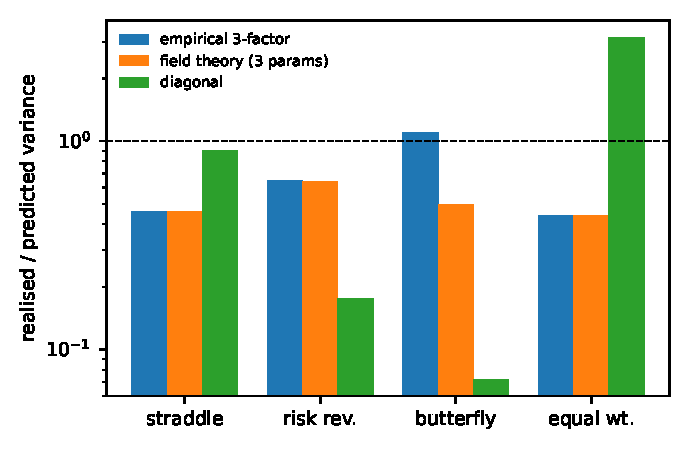
\includegraphics[width=.66\linewidth]{figures/fig3_oos.pdf}
\caption{Out-of-sample variance ratios (log scale; dashed line = perfect).
Field theory and the empirical 3-factor model agree to $\le1\%$ everywhere
except the butterfly, which isolates the mode-4--5 residual.}
\label{fig:oos}
\end{figure}

\section{Discussion}
\label{sec:discussion}

\textbf{What holds.} Within its observable band, the SPX smile's daily dynamics are quantitatively consistent with a two-component structure: an external volatility-level factor (91.5\% of change variance, uniform in $z$, plausibly containing the gamma--theta carry and market-wide repricing) riding on a stiff membrane whose relaxation spectrum $\gamma_k=Dk^2+\kappa k^4$ has its diffusion-to-bending crossover at the edge of resolution. The structure is not merely descriptive: three calibrated parameters predict out-of-sample portfolio risk as well as a full empirical factor model wherever the model's one known residual is not isolated.

\textbf{What breaks, and where.} Pure diffusion is excluded outright. The homogeneous single-operator picture is excluded by spectral convexity. The composite's failure is localised to a mode-4--5 shelf, measured twice (spectral $z=-3.0$; butterfly $2.2\times$). Candidate mechanisms: a pinned or resonant structure in the put wing, fat-tailed shocks, slow parameter drift; are deliberately left for future work rather than fitted post hoc.

\textbf{Limitations.} (i) Resolution: 8 bins on $z\in[-1.15,1.10]$; deep wings and $k>8$ are invisible; claims are conditional on the band. (ii) Sufficiency, not uniqueness: other mechanisms could reproduce a finite-resolution spectrum; the claim is that the composite is the minimal sufficient extension tested. (iii) The measurement variable is $\Delta\sigma$, not delta-hedged P\&L; the difference is approximately rank-one and confined to mode~1's interpretation. (iv) Overall variance scale is non-stationary (COVID-in-train); the OOS test controls for it by design but a deployable risk model would rescale dynamically. (v) Maturity structure: this is a fixed-maturity (30-day) slice; the $\tau$-dimension and full 2D membrane are deferred. (vi) Rolling-window stability of the modes (in-sample stability is necessary but not sufficient) is the principal deferred robustness check.

\textbf{Methodological stance.} Every stage was validated against known ground truth before use (pipeline on synthetic data; forward model against simulation; error bars by block bootstrap respecting volatility clustering); predictions were stated before runs and graded after, including the supervisor-side failures (a predicted curvature mode~3, killed by an edge-tracking diagnostic; a predicted strong $D$--$\kappa$ degeneracy, not observed); and all measurement choices are recorded in a numbered decision log (Appendix~\ref{app:dlog}). Where the data contradicted expectation: the increment-law correction, the seven-bin panel artifact, the mode-3 boundary dipole, the hand-fit's rejection, the contradiction is reported as part of the result.

\appendix

\section{Decision log (abridged)}
\label{app:dlog}
\begin{description}
\item[D1] Strike from vendor \texttt{impl\_strike} (self-consistency; fewest assumptions).
\item[D2] OTM-only put/call stitching, $|\Delta|\le0.5$.
\item[D3] Calendar$\to$business days ($\times252/365$); omission shrinks $z$ by $\sim$17\%.
\item[D4] ATM-normalised $z$; usable window $[-1.15,1.10]$, 8 bins; 13.3\% of rows outside; hard error if $\sigma_{\mathrm{ATM}}$ absent.
\item[D5] Panel variable: daily $\Delta\sigma$ (stationarity; harness-matched; no hedging-frequency assumption); rank-one gamma--theta caveat on mode 1.
\item[D6] Phase-3 results: level and skew modes robust; mode 3 an edge artifact (node count unstable $2\to4$ under bin removal); slopes $p=2.99/3.20$, $p_{\mathrm{tail}}=2.53/2.64$.
\item[D7] Adjudication: diffusion falsified ($p_{\mathrm{tail}}\le1.87$); single $k^4$ operator profile-falsified (convexity); composite sufficient; aliasing control $n_{\mathrm{modes}}=n_z$; underflow guard re-derived.
\item[D8] Calibration: $D=0.69\,[0.29,1.25]$, $\kappa=0.011\,[0.006,0.020]$, $\sqrt m=2.64\,[2.25,3.35]$, $k^\ast=7.9\,[5.1,11.2]$; $\chi^2/\mathrm{dof}=3.6$; hand-fit rejected ($\Delta\chi^2=17.1$); sole residual mode-5 shelf ($z=-3.0$).
\item[D9] OOS test: field theory within 1\% of empirical 3-factor on level/straddle/risk-reversal; diagonal fails two-sided; butterfly over-predicted $2.2\times$, independently localising the D8 residual.
\end{description}

\section{Reproducibility}
All results derive from a public repository (\texttt{github.com/MichaelAafton/diffusion-modes-vol-surface}): a one-time WRDS pull script (raw data git-ignored under licence), the validated simulator and analytic forward model in \texttt{src/}, analysis scripts in \texttt{scripts/}, and a pytest suite that freezes the harness-recovery test, the increment-spectrum theory, and loader dtype guarantees. Randomness is seeded throughout; bootstrap and sweep settings are recorded in the scripts.

\begin{thebibliography}{9}
\bibitem{bouchaud} Bouchaud, J.-P.\ and Potters, M.\ (2003) \emph{Theory of financial risk and derivative pricing}. 2nd edn. Cambridge: Cambridge University Press.
\bibitem{cont} Cont, R.\ and da Fonseca, J.\ (2002) `Dynamics of implied volatility surfaces', \emph{Quantitative Finance}, 2(1), pp.~45--60.
\bibitem{gatheral} Gatheral, J.\ (2006) \emph{The volatility surface: a practitioner's guide}. Hoboken, NJ: John Wiley \& Sons.
\bibitem{lecoz} Le~Coz, V.\ and Bouchaud, J.-P.\ (2024) `Revisiting elastic string models of forward interest rates', \emph{Quantitative Finance}, 24, pp.~1561--1578.
\end{thebibliography}

\end{document}